\section{Results}\label{sec:results}

Results are reported in the order of the steps in Table~\ref{tab:steps}. Interval errors use the 500\,Hz ground truth and 49 reliable records unless stated; heart-rate results for Sweep~1 use the 44 records that were reliable in that sweep. Sweep~1 and Sweep~2 are reported separately and compared in Section~\ref{sec:drift}.

\subsection{Steps 1--3: does the chain work at all?}

\textbf{Step 1 (stand-in renderer).} The digitiser ran in 19\,s and returned all 12 leads, but the stand-in page matched none of its known layouts, so it fell back to a default and recovered only about 2.4\,s of lead~II, in which it found two heartbeats. That is too few to give a heart rate. The recovered amplitude was about one third of the true amplitude. The result was a connectivity proof, not an accuracy result: a picture went in and numbers came out.

\textbf{Step 2 (official renderer).} With the official tool's correctly formatted page, the digitiser recognised the layout with a low matching cost (0.094), recovered the full 10\,s, found 10 beats (the true count), and gave a heart rate of 63.8\bpm\ against a true 63.9\bpm. The recovered amplitude was about 90\,\% of the true amplitude. This showed that the Step~1 shortfall came from the stand-in picture and not from the digitiser.

\textbf{Step 3 (six records).} Five of six records were digitised accurately (Table~\ref{tab:step3}, Fig.~\ref{fig:step3}): the absolute heart-rate errors were 0.02--0.21\bpm\ (mean 0.09\bpm). One record (\texttt{00002}) returned only 2.5\,s of signal and no heart rate. Its rendered page looked normal, so the failure lay inside the digitiser. The digitiser's own layout-match cost was highest for this record (0.31, against 0.09--0.23 for the five that worked). One record is far too little to conclude that this cost predicts failure, but it is the kind of early-warning signal a later quality gate would need.

\begin{table}[ht]
\centering\small
\caption{Step~3: six-record validation on undamaged rendered pages (recomputed from the saved digitiser outputs). Recovered: seconds of the 10\,s record the digitiser returned.}\label{tab:step3}
\begin{tabular}{@{}lrrrr@{}}
\toprule
Record & True HR (bpm) & Digitised HR (bpm) & Error (bpm) & Recovered (s) \\
\midrule
\texttt{00001\_lr} & 63.9 & 63.8 & 0.07 & 10.0 \\
\texttt{00002\_lr} & 47.6 & no reading & -- & 2.5 \\
\texttt{00003\_lr} & 63.7 & 63.7 & 0.02 & 10.0 \\
\texttt{00004\_lr} & 74.7 & 74.9 & 0.21 & 10.0 \\
\texttt{00005\_lr} & 66.4 & 66.5 & 0.08 & 10.0 \\
\texttt{00006\_lr} & 83.1 & 83.0 & 0.08 & 10.0 \\
\bottomrule
\end{tabular}
\end{table}

\begin{figure}[ht]
\centering
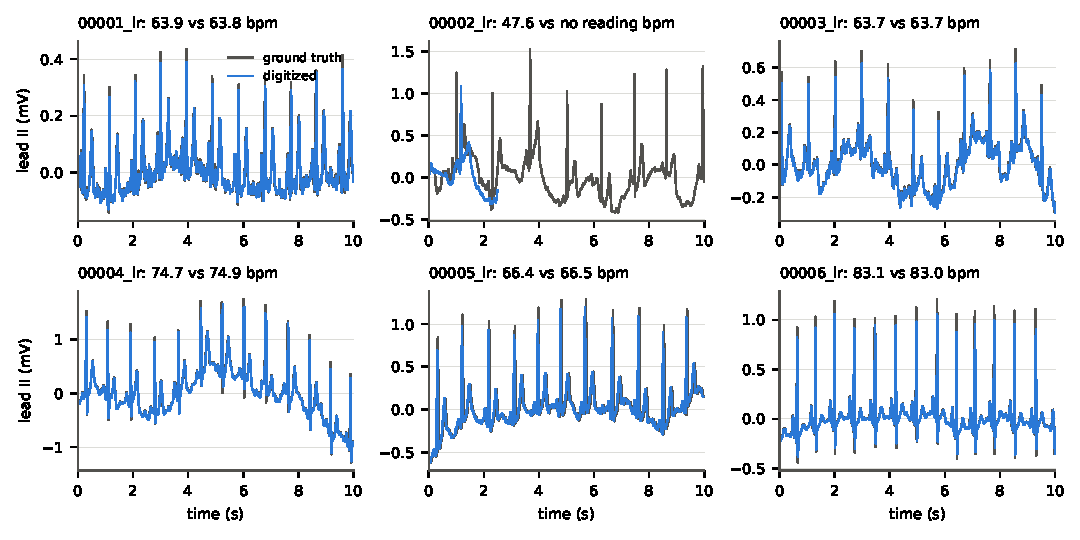
\includegraphics[width=\textwidth]{figures/fig_step3_validation.pdf}
\caption{Step~3 output: ground-truth (grey) and digitised (blue) lead~II for the six validation records on undamaged pages. Titles give true and digitised heart rate. Record \texttt{00002} shows the failure: only the first 2.5\,s were recovered.}\label{fig:step3}
\end{figure}

\subsection{Step 5: pilot}
The pilot (10 records, blur, 60 tests) ran at about 20.3\,s per image on a T4 GPU (about 120--150\,s on CPU) and showed heart-rate error rising with blur, from 0.09\bpm\ on clean images to 8.8\bpm\ at the heaviest blur in those 10 records. Its first digitiser crash (``weights only load failed'') looked like a PyTorch version problem. The cause was that \texttt{git-lfs} was not installed in the Colab image, so the model-weight files were small pointer stubs. Installing \texttt{git-lfs} before pulling fixed it. This full-sweep estimate (about 10.5 hours for 1{,}550 images) drove the scope reduction in Step~0.

\subsection{Step 6: Sweep 1 completion, cleaning and reliability}\label{sec:cleaning}
All 1{,}550 tests completed. The raw results file held 1{,}688 rows because 138 stray rows from earlier, larger scope settings had been written before the scope was reduced; after removing them there were 0 duplicates and every expected test was present. Roughly 35 minutes of progress had been made on CPU by mistake; the rest ran on a T4 GPU at 22--24\,s per image in about 5 hours. Several things went wrong along the way, each of which changed the design (Table~\ref{tab:problems}).

\begin{table}[ht]
\centering\small
\caption{Operational problems in Sweep~1 and what each changed.}\label{tab:problems}
\begin{tabularx}{\textwidth}{@{}>{\raggedright\arraybackslash}p{3.6cm}>{\raggedright\arraybackslash}X>{\raggedright\arraybackslash}p{4.4cm}@{}}
\toprule
Problem & What happened & Consequence \\
\midrule
Wrong scope ran & Step~3 copied every cached image, so the variant list covered 500 records, not 150; caught from the printed count (15{,}500 variants) & Variant list built only from the current sample \\
CPU by mistake (three times) & Newly uploaded notebooks default to CPU & Device printed and checked before trusting a run \\
GPU quota & Colab refused GPU after a few hours & Retried later; then a second account (study folder shared as editor) \\
Apparent data loss & A stale view suggested about 500 tests were lost; the file was complete & Verified saving (temporary file, atomic swap, backup, read-back check) \\
Two runs, one file & CPU and GPU runs worked on the same remaining tests and file & CPU run stopped as soon as the GPU run started \\
Hand-edited cells & Editing cells in the browser corrupted them repeatedly & Notebooks built locally, syntax-checked, dry-run on mock data, then uploaded \\
\bottomrule
\end{tabularx}
\end{table}

\textbf{Reliability in Sweep 1.} Of 1{,}550 tests, 163 (10.5\,\%) returned no heart rate, and in 154 of those no digitised signal was returned at all. The failures were concentrated in six records (unreadable in 18--31 of 31 versions: \texttt{00102}, \texttt{08150}, \texttt{13316}, \texttt{00053}, \texttt{18151}, \texttt{19059}); four of them (\texttt{00102}, \texttt{08150}, \texttt{13316}, \texttt{19059}) failed even on the clean image. Thirty-seven records never failed and seven failed once or twice (Fig.~\ref{fig:fig3}). Record \texttt{00102} also has no measurable ground-truth heart rate. These six records were excluded from Sweep~1 degradation analyses, leaving 44 reliable records.

\begin{figure}[ht]
\centering
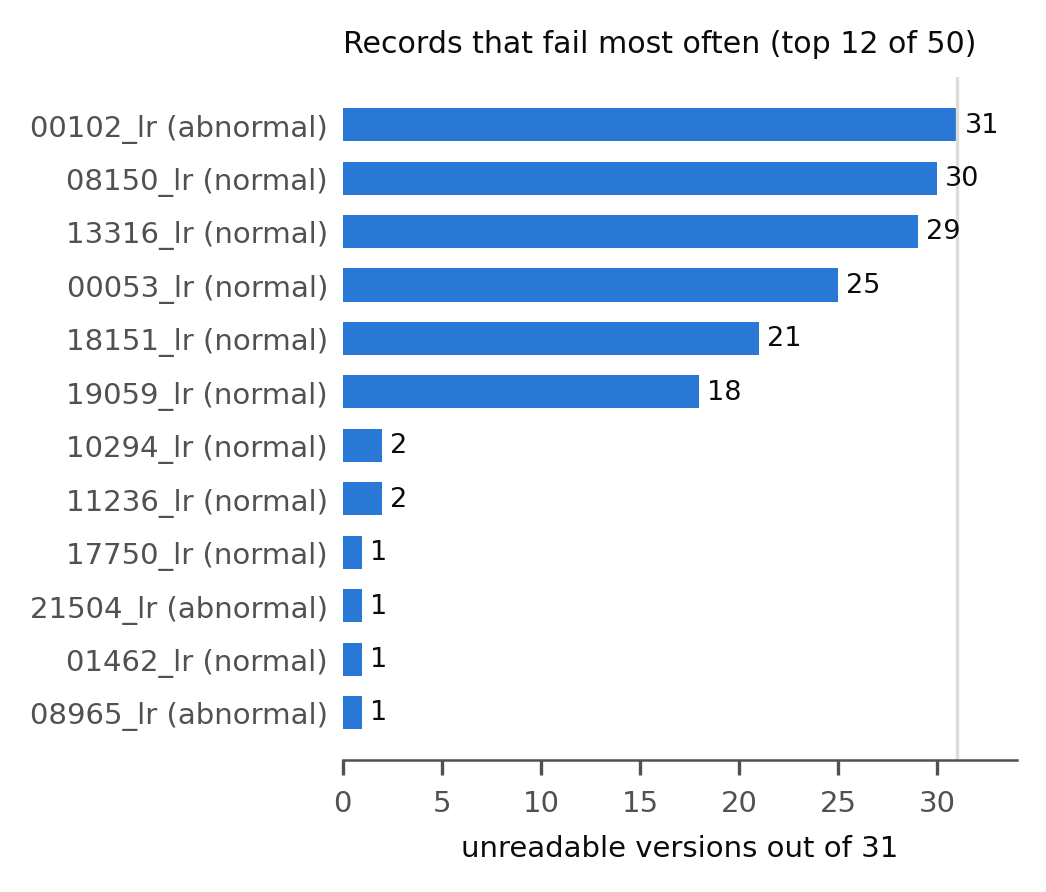
\includegraphics[width=0.55\textwidth]{figures/fig3_unreadable_records.png}
\caption{Sweep~1: the 12 records (of 50) with the most unreadable versions out of 31. Six fail in most versions, four of them on the clean image too. Sweep~2 did not reproduce this pattern (Section~\ref{sec:drift}).}\label{fig:fig3}
\end{figure}

\subsection{Step 7: Sweep 1, heart rate}\label{sec:hr1}
On clean images the mean heart-rate error was 0.52\bpm\ (median 0.13\bpm). Two of six axes showed a clear rise with severity (Fig.~\ref{fig:fig1}). For blur the mean error rose from 0.41\bpm\ (level 1) to 2.90\bpm\ (level 5), with a median of 0.12 to 1.64\bpm. For low resolution the error stayed near baseline through level~4 (median 0.11--0.20\bpm) and then jumped at level~5 to a mean of 7.72\bpm\ and a median of 2.36\bpm, with 41\,\% of readings more than 5\bpm\ off. Tilt, JPEG compression, grid contrast and uneven lighting stayed within the baseline band (mean error $\le$1.2\bpm\ at every level).

\begin{figure}[ht]
\centering
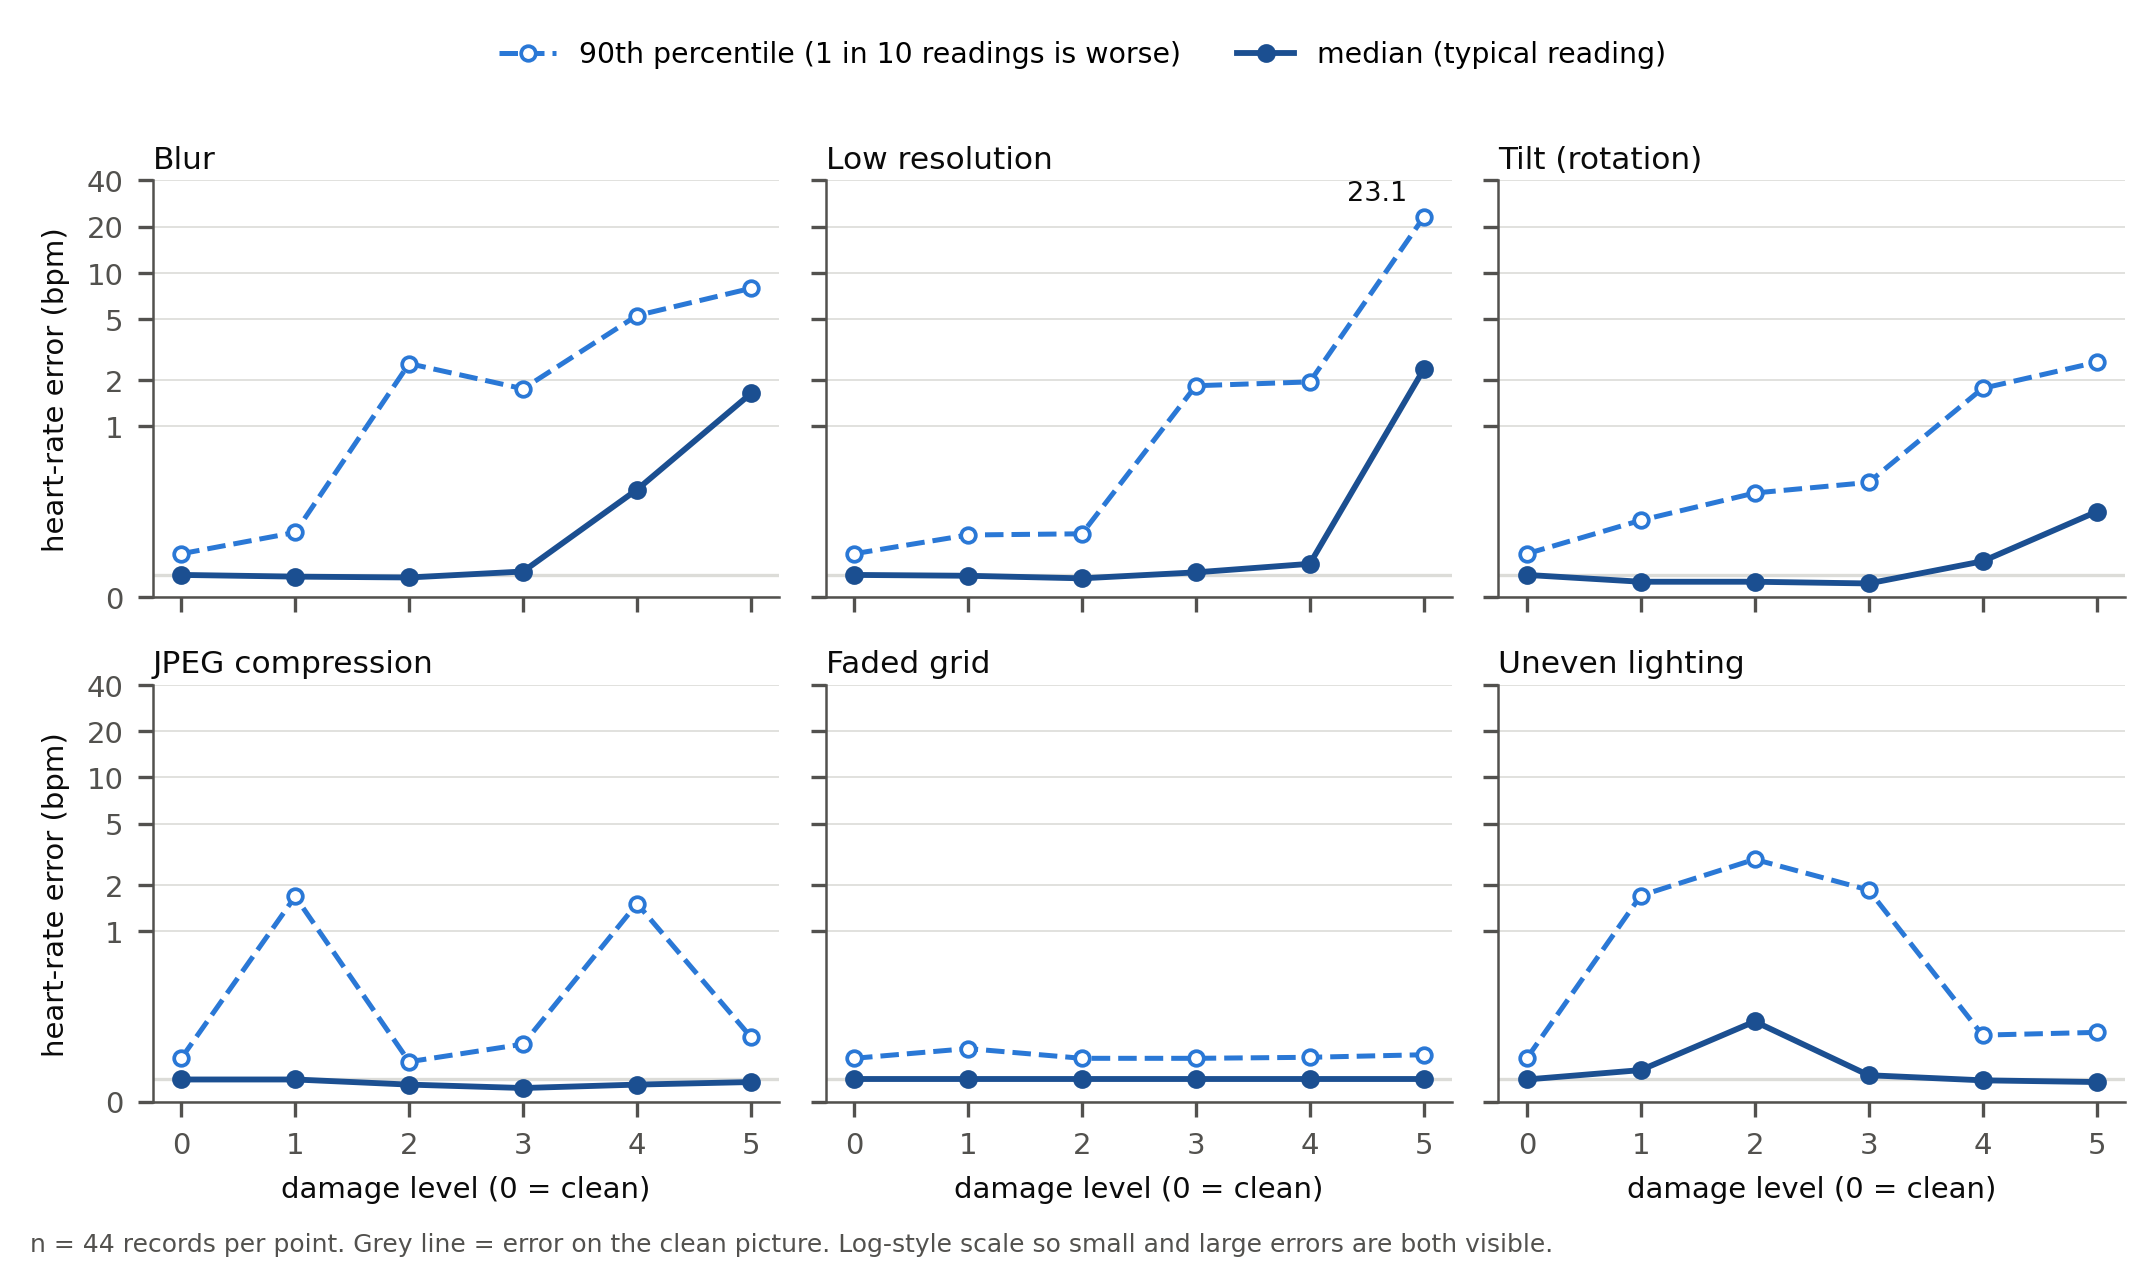
\includegraphics[width=\textwidth]{figures/fig1_hr_error_by_damage.png}
\caption{Sweep~1 (44 reliable records): absolute heart-rate error (symlog axis) against degradation level for each axis; solid line median, dashed line 90th percentile, grey line the clean-image median.}\label{fig:fig1}
\end{figure}

\textbf{Patient-facing outcome.} Only nine of the 44 reliable records have a slow or fast ground-truth heart rate (six slow, three fast) and can therefore show false reassurance. On clean images all 44 were read correctly. Across all degraded images nine readings were falsely reassuring; six were real (more than 10\bpm\ off) and three were boundary flips (for example 59.7 read as 60.0\bpm). \textbf{All six real events occurred at level~5, and only for two axes}: low resolution in 4 of 9 at-risk records (44\,\%, 95\,\% CI 19--73\,\%; errors 14--33\bpm) and blur in 2 of 9 (22\,\%, 95\,\% CI 6--55\,\%; errors about 15\bpm). No real event occurred at any other axis or at levels 1--4 of these two. Tilt caused a different failure: at level~5, 4 of 44 pictures (9\,\%) returned no reading (a silent drop) and none returned a wrong one (Fig.~\ref{fig:fig2}). With $n=9$ at risk the intervals are wide, so these counts describe a pattern, not a rate.

\begin{figure}[ht]
\centering
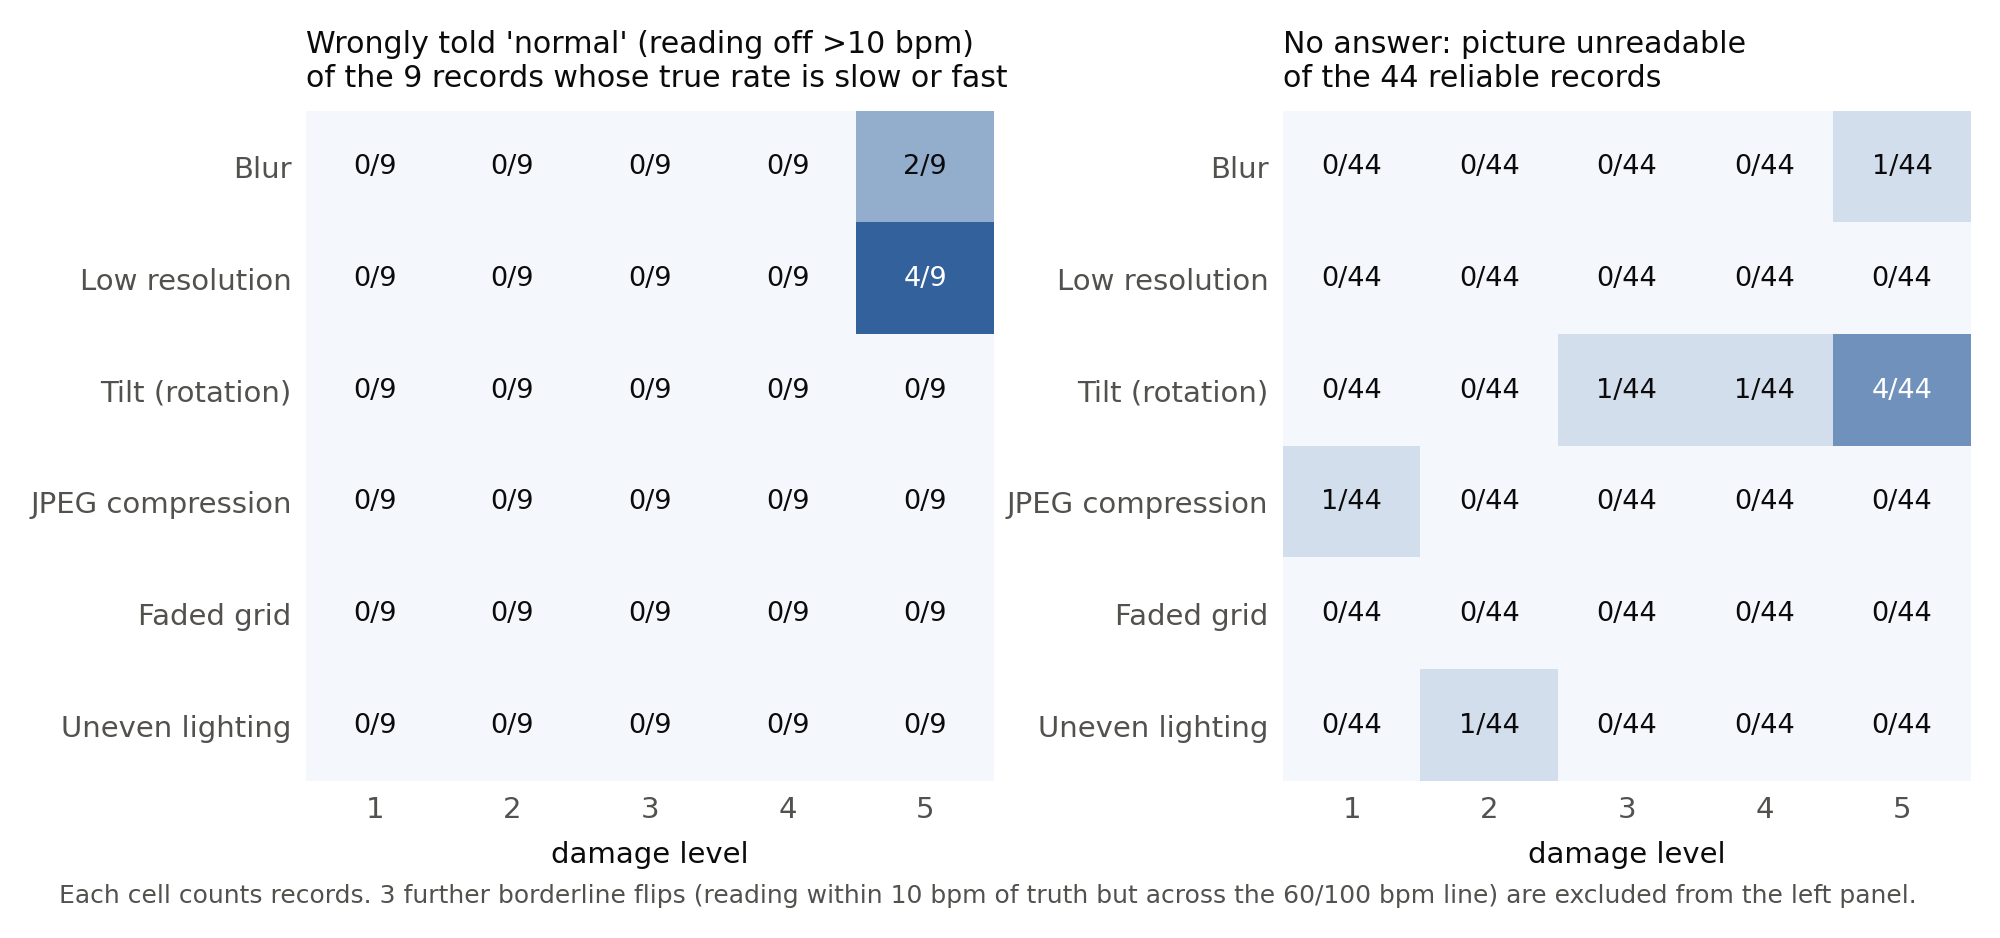
\includegraphics[width=\textwidth]{figures/fig2_false_reassurance_and_silent_drops.png}
\caption{Sweep~1. Left: of the nine records with a slow or fast true heart rate, how many were reported as normal (reading off by $>$10\bpm) at each axis and level. Right: of 44 reliable records, how many returned no reading.}\label{fig:fig2}
\end{figure}

\subsection{Step 8: Sweep 2 completion}
Sweep~2 completed all 1{,}550 tests overnight and produced a results file with 23 columns (Appendix Table~\ref{tab:dict}). Google Drive's mount misfiled checkpoint saves repeatedly: on two occasions stray copies of the results file appeared at the top level of the Drive instead of in the study folder (4 copies the first time, 19 the second). Each time, the copies were compared by row count with the file in the study folder, found to be older, smaller snapshots of the same data, and removed; no data were lost. The browser's view of the running notebook also stalled once on an accumulated-output replay problem while the kernel kept running (confirmed from Colab's session list), and was resolved by disconnecting the runtime, clearing outputs and restarting from the checkpoint. In this sweep 49 of 50 records were reliable: only \texttt{15192\_lr} failed badly (unreadable in 20 of 31 versions, but readable on its clean image). Of 1{,}550 tests, 30 (1.9\,\%) returned no heart rate and 41 (2.6\,\%) no QTc.

\subsection{Step 9: Sweep 2 analysis}

\subsubsection{Sweep 2 repeats the heart-rate findings}\label{sec:hr2}
Using the same rules as Sweep~1 on the 49 reliable records, 10 records have a slow or fast true heart rate (six slow, four fast; the fourth fast record, \texttt{08150}, was unreliable in Sweep~1). There were 10 falsely reassuring readings: \textbf{six real, all at level~5 (blur 2, low resolution 4)}, with errors of 14.2--33.3\bpm, and four boundary flips. The clean-image mean error was 0.53\bpm\ (median 0.13\bpm); at level~5 the blur mean was 3.30\bpm\ (median 1.65\bpm) and the resolution mean 7.84\bpm\ (median 2.54\bpm), with 42.9\,\% of resolution-5 readings more than 5\bpm\ off. Tilt level~5 produced 5 silent drops of 49. On the clean images, the heart-rate band matched ground truth in 48 of 49 records. The headline pattern is therefore the same in both sweeps; as Section~
ef{sec:drift} shows, this is a repeat of the same tests, not an independent replication.

\subsubsection{Agreement on clean images}
On undamaged images heart rate agreed closely with ground truth: bias $+0.26$\bpm, 95\,\% limits of agreement $-3.1$ to $+3.6$\bpm, mean absolute error 0.53\bpm\ (Table~\ref{tab:ba}, Fig.~\ref{fig:ba}). Two records (of 49) differed by more than 5\bpm. Intervals agreed much less well: mean absolute errors were 11.0\,ms (PR), 21.2\,ms (QRS), 19.3\,ms (QT) and 22.1\,ms (QTc), with systematic biases of $-7.3$, $+19.4$, $+13.3$ and $+15.4$\,ms; digitised QRS is longer than ground truth, which is consistent with a thicker reconstructed trace, although we did not test that explanation.

\begin{table}[ht]
\centering\small
\caption{Agreement on clean images (digitised minus ground truth; intervals against 500\,Hz ground truth; $n=49$ reliable records). LoA: 95\,\% limits of agreement; MAE: mean absolute error.}\label{tab:ba}
\begin{tabular}{@{}lrrrrr@{}}
\toprule
Measure & Bias & SD & LoA low & LoA high & MAE \\
\midrule
HR (bpm) & +0.26 & 1.70 & -3.1 & +3.6 & 0.53 \\
PR (ms) & -7.29 & 13.08 & -32.9 & +18.4 & 11.04 \\
QRS (ms) & +19.35 & 21.23 & -22.3 & +61.0 & 21.15 \\
QT (ms) & +13.29 & 24.77 & -35.3 & +61.8 & 19.26 \\
QTc (ms) & +15.44 & 28.02 & -39.5 & +70.3 & 22.10 \\
\bottomrule
\end{tabular}
\end{table}

\begin{figure}[ht]
\centering
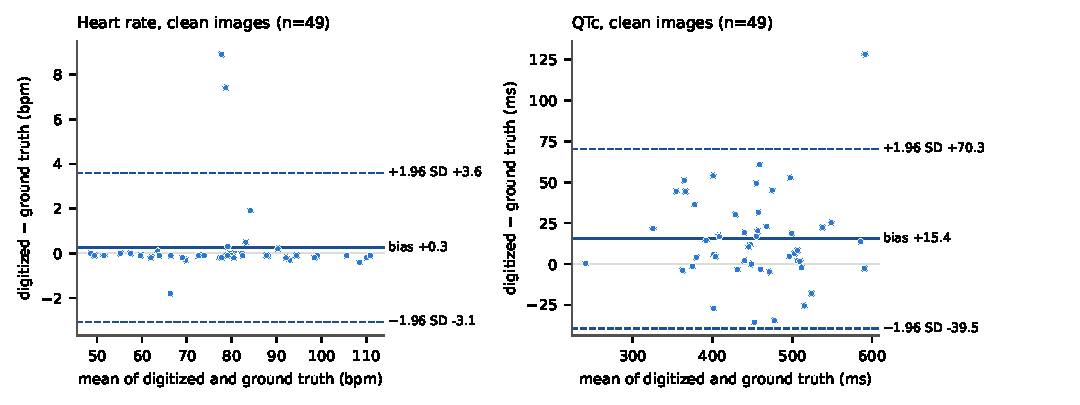
\includegraphics[width=\textwidth]{figures/fig_bland_altman_clean.pdf}
\caption{Bland--Altman plots on clean images. Left: heart rate. Right: QTc against the 500\,Hz ground truth. Solid line: bias; dashed lines: 95\,\% limits of agreement.}\label{fig:ba}
\end{figure}

\subsubsection{Interval error against degradation}\label{sec:intervalerr}
The interval results mirror heart rate (Table~\ref{tab:intervals}, Fig.~\ref{fig:intervals}). For blur, the median QTc error rose from 17.3\,ms on clean images to 24.4, 45.0, 77.8 and 90.8\,ms across levels 2--5; QRS from 16.2 to 117.6\,ms; QT from 12.9 to 77.0\,ms. For low resolution the rise was later and steeper (QTc 35.1\,ms at level 4, 73.0\,ms at level 5). \textbf{PR was the exception}: its median error rose only from 9.1 to at most 22.2\,ms and did not increase monotonically. The other four axes stayed close to the clean-image baseline (Table~\ref{tab:flat}); the largest deviation was tilt at level~5, where the median QTc error was 26.8\,ms against 17.3\,ms on clean images, which was not significant after correction.

\begin{table}[ht]
\centering\small
\caption{Median absolute error against ground truth, by level, for the two axes that matter (49 reliable records; intervals against 500\,Hz ground truth; heart rate in bpm, intervals in ms). Level 0 is the clean image.}\label{tab:intervals}
\begin{tabular}{@{}llrrrrr@{}}
\toprule
Axis & Level & HR & PR & QRS & QT & QTc \\
\midrule
Clean & 0 & 0.13 & 9.1 & 16.2 & 12.9 & 17.3 \\
\midrule
Blur & 1 & 0.12 & 9.8 & 17.7 & 14.1 & 17.3 \\
 & 2 & 0.15 & 10.2 & 34.8 & 23.3 & 24.4 \\
 & 3 & 0.16 & 16.4 & 66.5 & 40.7 & 45.0 \\
 & 4 & 0.64 & 22.2 & 107.3 & 67.9 & 77.8 \\
 & 5 & 1.65 & 16.6 & 117.6 & 77.0 & 90.8 \\
\midrule
Low resolution & 1 & 0.12 & 8.2 & 17.5 & 12.9 & 16.2 \\
 & 2 & 0.12 & 10.5 & 18.0 & 17.5 & 21.7 \\
 & 3 & 0.15 & 11.3 & 25.2 & 19.6 & 20.7 \\
 & 4 & 0.21 & 13.3 & 41.1 & 30.2 & 35.1 \\
 & 5 & 2.54 & 17.4 & 77.1 & 65.1 & 73.0 \\
\bottomrule
\end{tabular}
\end{table}
\begin{table}[ht]
\centering\small
\caption{The four axes that did not matter: lowest--highest of the five level medians of absolute error (49 reliable records). Compare the clean-image medians in Table~\ref{tab:intervals}.}\label{tab:flat}
\begin{tabular}{@{}lccccc@{}}
\toprule
Axis & HR (bpm) & PR (ms) & QRS (ms) & QT (ms) & QTc (ms) \\
\midrule
Tilt & 0.08--0.55 & 8.3--10.0 & 14.7--21.9 & 11.1--19.9 & 12.8--26.8 \\
JPEG & 0.08--0.14 & 7.3--9.1 & 15.3--18.4 & 11.6--14.0 & 12.8--16.9 \\
Grid contrast & 0.12--0.13 & 7.9--9.2 & 15.4--16.2 & 12.0--13.2 & 16.6--17.3 \\
Uneven lighting & 0.12--0.45 & 7.9--10.9 & 14.9--16.0 & 11.3--14.6 & 14.3--19.5 \\
\bottomrule
\end{tabular}
\end{table}

\begin{figure}[ht]
\centering
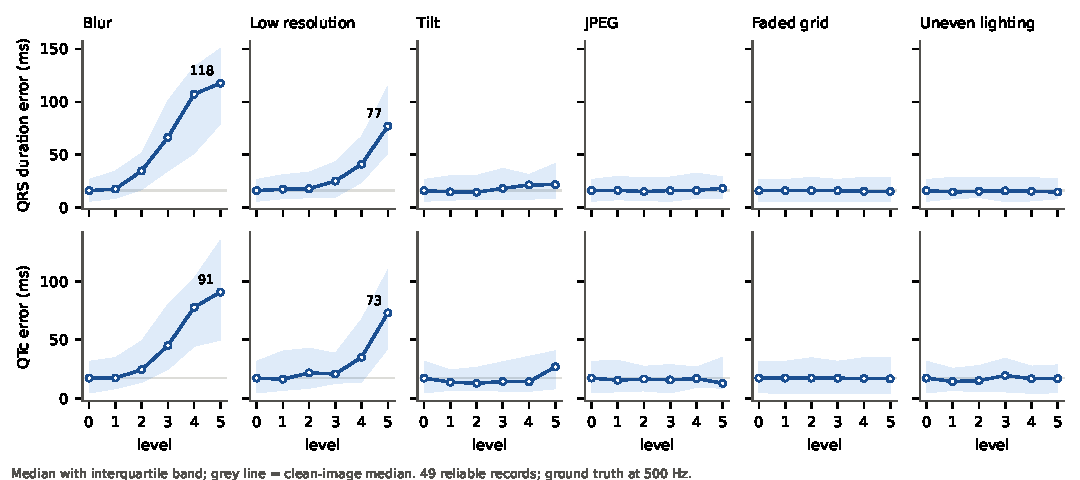
\includegraphics[width=\textwidth]{figures/fig_interval_error_by_level.pdf}
\caption{Sweep~2: QRS-duration and QTc absolute error against degradation level for each axis (median and interquartile band; grey line is the clean-image median). Numbers mark the level-5 median for the two axes that matter.}\label{fig:intervals}
\end{figure}

\textbf{Statistics.} Against each record's own clean image, blur produced significant increases (Holm-adjusted $p<0.05$) from level~2 for QRS, QT and QTc and from level~3 for PR; low resolution from level~3 for QT and QTc, level~4 for QRS and level~5 for PR (Table~\ref{tab:tests}). The effect sizes were large: at level~5, the median excess QTc error was 63.8\,ms for blur and 52.3\,ms for resolution, and the median excess QRS error 98.1 and 57.0\,ms. A few other cells were statistically significant with negligible effects, which illustrates why effect size matters: in heart rate, JPEG level~3 ($-0.03$\bpm), tilt level~4 ($+0.06$\bpm) and lighting level~2 ($+0.24$\bpm) were significant, and tilt level~5 raised QRS error by 3.9\,ms. None of these is clinically meaningful.

\begin{table}[ht]
\centering\small
\caption{Paired comparison of each degraded level with the same record's clean image (Wilcoxon signed-rank, Holm-corrected over 30 comparisons per metric). ``Lowest sig.\ level'' is the lowest level with adjusted $p<0.05$; the effect is the median paired excess error at level~5 (bpm for HR, ms otherwise).}\label{tab:tests}
\begin{tabular}{@{}llccc@{}}
\toprule
Metric & Axis & Lowest sig.\ level & Effect at level 5 & Significant cells (of 5) \\
\midrule
HR & Blur & 4 & +1.46 & 2 \\
 & Low resolution & 5 & +2.45 & 1 \\
 & Tilt & 4 & +0.31 & 2 \\
 & JPEG & 3 & +0.00 & 1 \\
 & Grid contrast & none & +0.00 & 0 \\
 & Uneven lighting & 2 & -0.01 & 1 \\
\midrule
PR & Blur & 3 & +8.01 & 3 \\
 & Low resolution & 5 & +7.23 & 1 \\
 & Tilt & none & +1.65 & 0 \\
 & JPEG & none & +0.10 & 0 \\
 & Grid contrast & none & +0.00 & 0 \\
 & Uneven lighting & none & +0.30 & 0 \\
\midrule
QRS & Blur & 2 & +98.05 & 4 \\
 & Low resolution & 4 & +57.00 & 2 \\
 & Tilt & 5 & +3.90 & 1 \\
 & JPEG & none & +2.20 & 0 \\
 & Grid contrast & none & +0.00 & 0 \\
 & Uneven lighting & none & +0.10 & 0 \\
\midrule
QT & Blur & 2 & +57.52 & 4 \\
 & Low resolution & 3 & +50.50 & 3 \\
 & Tilt & none & +3.95 & 0 \\
 & JPEG & none & +1.10 & 0 \\
 & Grid contrast & none & +0.00 & 0 \\
 & Uneven lighting & none & +0.30 & 0 \\
\midrule
QTc & Blur & 2 & +63.79 & 4 \\
 & Low resolution & 3 & +52.30 & 3 \\
 & Tilt & none & +4.30 & 0 \\
 & JPEG & none & +1.70 & 0 \\
 & Grid contrast & none & +0.00 & 0 \\
 & Uneven lighting & none & +0.17 & 0 \\
\bottomrule
\end{tabular}
\end{table}

\subsubsection{QTc patient-facing outcome (exploratory)}\label{sec:qtcoutcome}
Twenty records have a truly prolonged QTc under the sex-specific threshold. A first, naive count of falsely reassuring QTc classifications found 26 events. Twenty of these were on records whose \emph{own clean image} was already misclassified, so no degradation was needed to produce them; the interval error floor alone moved an already borderline QTc across the threshold. Counting them as degradation effects would be wrong. Requiring that the record be classified correctly on its clean image, and the error exceed 10\,ms, leaves \textbf{6 real events among 19 usable at-risk records}: blur level~2 (1), low resolution level~2 (1), tilt levels~4 and~5 (1 each), and uneven lighting levels~1 and~3 (1 each). Each cell has at most one event, so the per-cell Wilson intervals are very wide (a single event in 19 records: 5\,\%, 95\,\% CI 1--25\,\%), and the events do not concentrate at the most severe levels as the heart-rate events do. On clean images the QTc outcome was correct in 42 of 49 records, a false alarm in six and a false reassurance in one. We regard this as an exploratory, underpowered signal, not as a second confirmed false-reassurance channel.

\subsubsection{Ground truth sampling rate}\label{sec:gt500}
The sweep computed ground-truth intervals from PTB-XL's 100\,Hz records (10\,ms per sample), whereas the digitised signal is at 1{,}000\,Hz. Recomputing the ground truth from the 500\,Hz versions of the same records reduced the clean-image mean absolute error of the digitised values from 18.5 to 11.0\,ms (PR), 32.1 to 21.2\,ms (QRS), 22.7 to 19.3\,ms (QT) and 25.0 to 22.1\,ms (QTc), and the clean-image median QTc error from 20.2 to 17.3\,ms. The ground truth itself was unstable across sampling rates: for the same records, 100\,Hz and 500\,Hz ground-truth QT differed by a mean absolute 10.6\,ms, QTc by 13.2\,ms and QRS by 15.2\,ms. Even the ground-truth heart rate differed by a mean absolute 0.75\bpm\ between the two rates, which is larger than the digitiser's own clean-image heart-rate error, so heart-rate agreement is limited by ground-truth uncertainty as much as by the digitiser. The qualitative conclusions did not change with the 500\,Hz ground truth: blur and resolution still raised interval error steeply, the other axes stayed flat, and the corrected QTc analysis again gave six real events. \textbf{Part of the interval error floor is therefore an artefact of our own ground truth, and part is not.}

\subsubsection{Diagnostic superclass}
Table~\ref{tab:class} shows median errors by class. Heart-rate error was small on clean images in every class ($\le$0.2\bpm\ except the single record with no superclass), rose at level~5 of both axes in every class, and was largest under low resolution for MI (7.4\bpm, 4 records). QTc error at level~5 of blur ranged from 67 to 124\,ms across classes. Class sizes are 1--23, so no class is shown to be more or less vulnerable than another.

\begin{table}[ht]
\centering\small
\caption{Median absolute error by diagnostic superclass on clean images and at level~5 of blur and of low resolution. Classes have 1--23 records, so this is descriptive only.}\label{tab:class}
\begin{tabular}{@{}lrrrrrrr@{}}
\toprule
 & & \multicolumn{3}{c}{HR (bpm)} & \multicolumn{3}{c}{QTc (ms)} \\
\cmidrule(lr){3-5}\cmidrule(lr){6-8}
Class & Records & Clean & Blur 5 & Res.\ 5 & Clean & Blur 5 & Res.\ 5 \\
\midrule
No superclass & 1 & 7.4 & 7.7 & 11.9 & 18.0 & 61.1 & 3.5 \\
CD & 5 & 0.2 & 1.7 & 1.8 & 3.5 & 66.9 & 56.4 \\
HYP & 9 & 0.1 & 1.6 & 3.8 & 22.3 & 101.9 & 58.6 \\
MI & 4 & 0.2 & 2.9 & 7.4 & 27.7 & 99.0 & 66.0 \\
NORM & 23 & 0.1 & 1.1 & 2.9 & 19.1 & 88.3 & 82.3 \\
STTC & 7 & 0.1 & 2.0 & 0.7 & 13.6 & 124.0 & 78.5 \\
\bottomrule
\end{tabular}
\end{table}

\subsection{Reproducibility between the two sweeps}\label{sec:drift}
Sweeps 1 and 2 used the same 50 records, the same rendered pages and the same degradation code, five days apart, but an unpinned digitiser. Table~\ref{tab:repro} compares what can be compared from the recorded summaries.

\begin{table}[ht]
\centering\small
\caption{Sweep~1 against Sweep~2. Sweep~1 figures are from the recorded Sweep~1 summary; Sweep~2 figures were recomputed from its results file.}\label{tab:repro}
\begin{tabular}{@{}lrr@{}}
\toprule
 & Sweep 1 & Sweep 2 \\
\midrule
Reliable records & 44 & 49 \\
Unreadable tests (no heart rate) & 163 (10.5\,\%) & 30 (1.9\,\%) \\
Records unreadable even on the clean image & 4 & 0 \\
Records with slow or fast true heart rate & 9 & 10 \\
Real heart-rate false reassurance events & 6 & 6 \\
\quad blur, level 5 & 2 & 2 \\
\quad low resolution, level 5 & 4 & 4 \\
Boundary flips & 3 & 4 \\
Silent drops, tilt level 5 & 4 of 44 & 5 of 49 \\
Clean-image heart-rate error, mean (median), bpm & 0.52 (0.13) & 0.53 (0.13) \\
Blur level 5, mean (median), bpm & 2.90 (1.64) & 3.30 (1.65) \\
Low resolution level 5, mean (median), bpm & 7.72 (2.36) & 7.84 (2.54) \\
\bottomrule
\end{tabular}
\end{table}

We compared the two sweeps test by test, matching all 1{,}550 variants by identifier (script \texttt{v1\_v2\_per\_test\_comparison.py}, using the Sweep~1 results file). The ground-truth heart rate was identical in all 1{,}397 tests where both had one. Of the 1{,}367 tests that produced a heart rate in both sweeps, 1{,}357 (99.3\,\%) agreed to within 0.15\bpm; the other ten differed by 0.2--5.9\bpm\ (largest: \texttt{13618\_lr} at resolution level~4, 105.2 against 99.3\bpm), and on clean images the two sweeps agreed to 0.1\bpm\ or better. The same nine tilt, blur, JPEG and lighting tests were unreadable in both. The six real false-reassurance events are \emph{the same six tests} in both sweeps (\texttt{10811} at resolution~5; \texttt{15049} at blur~5 and resolution~5; \texttt{16637} at resolution~5; \texttt{20052} at blur~5 and resolution~5).

The two sweeps differed in only seven records. Six records that failed in Sweep~1 (\texttt{00102}, \texttt{08150}, \texttt{13316}, \texttt{19059}, which failed even on the clean image, and \texttt{00053}, \texttt{18151}, which failed on most versions) became readable in Sweep~2 (18--31 tests each), and \texttt{15192} went the other way (20 tests). Together these explain all 173 tests whose readable status changed. Because the digitiser was cloned afresh in each session without pinning a commit, the most likely explanation is that the upstream tool changed between the sweeps, but we cannot confirm this, because the versions were not recorded.

Two conclusions follow. First, \textbf{Sweep~2 is a repeat, not an independent replication.} The rendered pages, the degradation code and the digitiser behaviour on 43 of the records are effectively deterministic, so the same tests give the same numbers. Agreement between the sweeps shows that the pipeline is computationally reproducible; it adds no new evidence that the effect would appear on other records or images. The evidence for the effect remains that of a single 50-record sample. Second, which records fail is a property of a tool build, not of an image: a study that excludes records by name (as Sweep~1 did) is describing one build.
